%liste des modules réalisés
%Preuve du fonctionnement de chaque modules

\subsection{Traitement des documents avec OCR}



\subsection{Récupération des données d'importance}



\subsection{Taxonomie}%Martin
\subsubsection{Approche par Word2Vec\label{word2vecReal}}
Pour extraire la taxonomie des documents, nous avons débuté par une approche basée sur des \textit{\gls{embed}} construits grâce à un réseau Word2Vec entrainé sur un corpus français.
Idéalement, ce réseau nous permettrait d'obtenir des taxonomies en comparant les mots du documents avec ceux présent dans la liste de taxonomies (sous forme de vecteurs), et d'ajouter les mots dont la distance, définie en (~\ref{eq:distCosine}), est sous un seuil.
Cette approche, ne nécessitant pas de corpus annoté semblait correspondre à nos besoins, même si il n'existe pas de cas dans la littérature scientifique ou elle a été appliquée avec succès. %Réecrire...


Les failles décelées par l'implémentation de cette méthode sont les suivantes.

Premièrement, le temps d'exécution de cette méthode pour un seul document était bien trop long pour imaginer un test sur nos 431 documents.
En effet, un document administratif est par nature très verbeux, et donc long.

La majorité du texte ne nous est cependant pas nécessaire pour une analyse taxonomique; 
il sert en effet a donner un contexte précis pour le lecteur et ne donne pas forcément plus d'information concernant le sujet du document en lui même que le titre du document en question, qui contient souvent toutes les informations taxonomiques nécéssaires. 


Deuxièmement, nous n'avons pas pu obtenir les résultats taxonomiques escomptés.
Le principal obstacle venant du fait que les mots de la taxonomie peuvent être en fait des phrases, ou tout du moins de multiples mots dont les sens ne sont pas forcément corrélés.

Par exemple, `Outre mer', `fromage au lait cru', `Pays de la Loire', \ldots et le très utilisé `Délégation de signature' sont des termes de la taxonomie composés de plusieurs mots dont le sens n'est pas proche.

Word2Vec, que nous utilisions pour obtenir les \textit{embeddings}, ne fonctionne bien que pour des mots uniques et pas sur des \textit{groupes de mots} ou \textit{n-grammes}.
Doc2vec, qui lui peut fonctionner sur des n-grammes, voir des paragraphes ou documents entiers, a besoin d'être entrainé sur des documents labellisés qui lui apporteront le contexte nécessaire pour former des \textit{embeddings} cohérents.


Cependant, la taxonomie donne un context très difficile a analyser pour un programme.
Il s'agit seulement d'une liste de mots et de phrasez ordonnée sous la forme d'un arbre (voir figure~\ref{fig:tree}).
Cette disposition rend l'utilisation d'un Doc2Vec très inconventionnelle, et les test que nous avons mené n'ont pas donné de résultats.


Nous tout d'abord amélioré la rapidité d'exécution en précalculant les vecteurs de la taxonomie.
Initialement, nous itérions simplement sur la liste de taxonomies, et calculions les \textit{embeddings} à la volée.
En calculant les vecteurs \textit{embedding} avant même l'exécution du module de détection de taxonomie, avons économisé une dizaine de secondes par documents.
Ensuite, plutôt que de traiter l'intégralité du texte avec Word2Vec, nous avons utilisé que les titres des arrêtés du RAA, qui peuvent constituer a eux seuls un résumé du RAA\@.
Ainsi, la quantité de texte a analyser est grandement réduite et une dizaine de secondes d'analyse supplémentaire sont gagnées par documents.

Pour essayer de contrer le problème des mauvais résultats, nous avons transformé chaque mots de la phrase en sa racine par le procédé dit la \textit{lemmatisation} à l'aide de la librairie Spacy\cite{spacy}.
Nous avons également filtré les \textit{stopwords} du texte a analyser.
Les \textit{stopwords} sont des mots très fréquemment dans les phrases, comme les déterminants, transformant la phrase `médecine physique et de réadaptation' en `médecine physique réadaptation'.
On utilise ensuite un Word2Vec sur chaque mot de la taxonomie est du titre pour obtenir plusieurs vecteurs.
Pour obtenir un seul vecteur que nous comparerons avec les mots du documents, nous effectuons un simple moyennage entre les valeurs de chaque mots de la phrase.


Ces modifications ont améliorés significativement les performances en temps du programme et la pertinence des taxonomies obtenues.
Cependant, les taxonomies obtenues a l'aide de ce système n'étais pas encore d'une qualité suffisante pour nos standards.
Les taxonomies monotermes étaient bien mieux détectées mais les multitermes restaient inutilisées.


Ce dysfonctionnement est du a la manière dont nous utilisons les vecteurs de mots produit par Word2Vec: une comparaison simple, ne donnant qu'une métrique de similarité ne suffit pas a établir un contexte suffisant pour ajouter des taxonomies sensées.
En effet, si un mot dans un titre et un mot dans la taxonomie sont identiques, alors leur métrique sera forcément faible (ils seront considérés comme ayant un sens proche), même si ces deux mots sont utilisés différemment dans le contexte actuel.
On peut prendre l'exemple du terme `montant': il peut avoir la signification d'un nombre, une action, un élément d'une porte, \ldots

On se retrouve alors a obtenir une grande quantités de termes taxonomiques qui ne sont pas pertinentes.
De plus, la question de la rapidité d'analyse n'as pas pu être totalement élucidée, même avec un prétraitement des vecteurs et l'utilisation des titres plutôt que du texte entier.
Pour un seul document, on pouvait avoir jusqu'à plusieurs dizaines de secondes de calcul pour la seule taxonomie.
Même si l'optimisation n'était pas une priorité dans ce projet, il devenait évident que cette approche ne fonctionnerait pas dans les délais impartis.


\subsubsection{Approche par détection de mots commun}
La solution donnant les meilleurs résultats fut d'extraire les titres d'arrêtées administratifs, qui sont les principaux constituants des RAA a classer, les traiter par lemmatisation et élimination des stopwords, puis d'effectuer une recherche des mots communs dans la taxonomie.
Si un terme lemmatisé de la taxonomie se trouve dans le titre de l'article administratif, alors celui ci est ajouté au document.
Cette solution est non seulement bien plus simple, mais permet également de vérifier la qualité des résultats plus aisément qu'à l'aide d'un \textit{embedding}, et elle est bien plus rapide, permettant l'analyse d'un document entier en quelques secondes à peine.

\begin{figure}[h!]
  \centering
  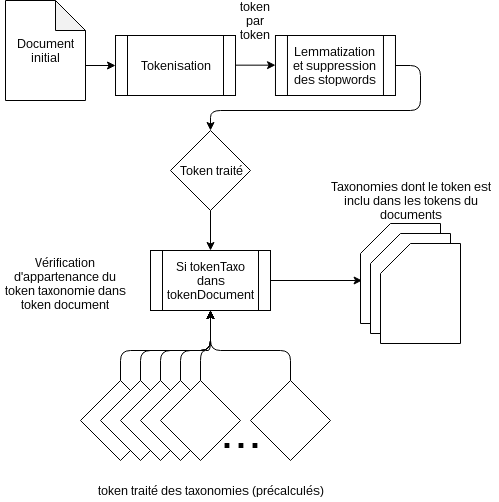
\includegraphics[width=0.7\textwidth]{diagFinalTaxo.png}
	\caption[]{Schéma fonctionnel du module d'assignement taxonomique final}
	\label{taxoFinal}
\end{figure}

\subsubsection{Parcours de l'arbre taxonomique}
\begin{figure}[h!]
  \centering
  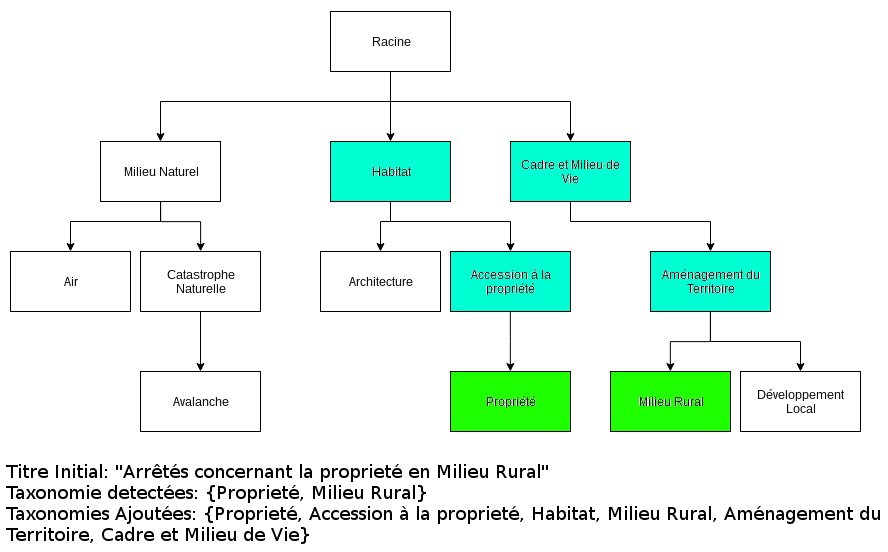
\includegraphics[width=\textwidth]{remontageArbre.png}
	\caption[]{Représentation de la technique de parcours d'arbre utilisée pour obtenir plus de taxonomies}
	\label{fig:tree}
\end{figure}


Pour obtenir une taxonomie plus vaste et contextuelle, nous prenons également en compte la structure de l'arbre taxonomique.
En effet, celle ci se présente sous forme d'un arbre dont un exemple de la structure est présenté en figure~\ref{fig:tree}. 
Chaque sections possède des sous sections, qui permettent un affinage et une grande précision dans la classification.

L'idée centrale est de considérer que si un document possède comme taxonomie une feuille ou un noeud de cette arbre, alors il doit nécessairement posséder comme taxonomie tout les parents de ce noeud. 
Nous remontons alors jusqu'à la racine de l'arbre depuis le noeud de la taxonomie ayant été détectée, en ajoutant à la taxonomie du document tous les noeuds que nous rencontrons en chemin.
Cette approche nous permet d'obtenir une plus grande variété de taxonomie sans avoir a utiliser une analyse plus lourde sur le texte. 


\subsubsection{Classement des taxonomies}
En sortie, nous récupérons un grand nombre de taxonomie, données a la fois par la détection initiale et par le parcours de l'arbre.
Pour obtenir les taxonomies les plus représentatives du document, nous procédons ensuite a un classement des termes selon le nombre de fois ou chacune apparait dans le tableau des taxonomies.
Les taxonomies qui apparaissent souvent dans le document sont donc considérées comme plus `importante' que des taxonomies qui apparaissent plus rarement.

Le parcours d'arbre apportant une très grande quantité de nouveaux mots pour chaque taxonomies, il est donc nécessaire d'équilibrer ce système.
Pour se faire, nous appliquons un simple système de poids au taxonomies détectées: une taxonomie initiale aura un poids 100 supérieur a une taxonomie récupéré par le parcours d'arbre.

Cela permettra de garder uniquement les taxonomies les plus pertinentes.

